\begin{frame}[c]{Įrankiai ir mokymas}
    \begin{minipage}[t]{0.65\textwidth}
        CLIP mokymas:
        \begin{itemize}
            \item Kryžminės entropijos nuostolių funkcija
            \item 200 epochų
            \item Adam optimizatorius
            \item Mokymo žingsnio kosinusinio
kitimo planuotojas (\textit{cosine learning rate scheduler})
        \end{itemize}
        Difuzerio mokymas:
        \begin{itemize}
            \item Vidutinės
kvadratinės paklaidos nuostolių funkcija
            \item 200 epochų
            \item AdamW optimizatorius
            \item Mokymo žingsnio kosinusinio
kitimo planuotojas (\textit{cosine learning rate scheduler})
        \end{itemize}
    \end{minipage}
    \begin{minipage}[t]{0.29\textwidth}
        \begin{figure}
            \centering
            
\includegraphics[width=0.75\textwidth]{img/Google_Colaboratory_SVG_Logo.svg.png}
        \end{figure}
        \begin{figure}
            \centering
            
\includegraphics[width=0.75\textwidth]{img/Pytorch_logo.png}
        \end{figure}
        \begin{figure}
            \centering
            
\includegraphics[width=0.75\textwidth]{img/6308b84661b3e2a522f01468.png}
        \end{figure}
    \end{minipage}
\end{frame}
\begin{frame}[c]{Rezultatai}
    \begin{minipage}[t]{0.49\textwidth}
        \begin{itemize}
            \item CLIP modelis grafeno sintezės reakcijos rezultato nuotraukas klasifikuoja apytiksliai 16.67\% įsitikinimo (\textit{confidence}) lygmeniu.
            \item Difuzijos modelio optimali mokymo žingsnio reikšmė $3 * 10^{-4}$.
            \item Difuzijos modelio optimali mokymo žingsnio planuotojo     apšilimo reikšmė 0\%.
            \item Difuzijos modelio generuojamos nuotraukos panašios į mokymo duomenų nuotraukas.
        \end{itemize}
    \end{minipage}
    \begin{minipage}[t]{0.49\textwidth}
       \begin{figure}
            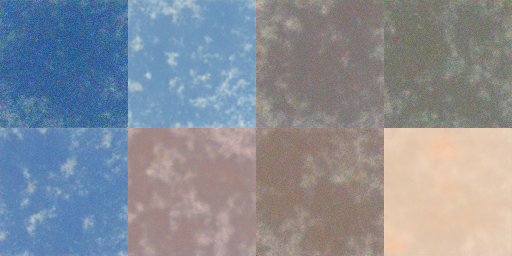
\includegraphics[width=1\textwidth]{img/graphene-diffuser-inference.png}
            \caption{Generatyviniu difuzijos modeliu sugeneruoti grafeno vaizdai}
        \end{figure}
    \end{minipage}
\end{frame}

\begin{comment}
\begin{frame}[c]{Visualization I}
    \begin{figure}
        
\includegraphics[width=1\textwidth]{img/sample1.png}
    \end{figure}
\end{frame}

\begin{frame}[c]{Visualization II}
    \begin{figure}
        \begin{tikzpicture}
            \node[inner sep=0pt] (A) at (0,0){
\includegraphics[width=.25\textwidth]{img/sample1.png}};
            \node[inner sep=0pt] (B) at (5,-4){
\includegraphics[width=.25\textwidth]{img/sample1.png}};
            \draw[<->,thick] (A.south east) -- (B.north west)node[midway,fill=white] {Some arrow};
            \node (A) at (6,0) {\(\displaystyle\left|
                \frac{
                    \left(\sum_{i=1}^n a_i^2\right) \cdot
                    \left(\sum_{i=1}^n b_i^2\right)
                }{ (\sum_{i=1}^n \underbrace{a_ib_i}_{\subnode{brace}{}})^2} \right| \geq 1\)};
        \end{tikzpicture}   
    \end{figure}        
\end{frame}
   
\begin{frame}[c]{Visualization III}    
    \begin{minipage}[t]{0.49\textwidth}
        \begin{itemize}
            \item XXX
            \item XXX
            \item XXX
        \end{itemize}
    \end{minipage}
    \begin{minipage}[t]{0.49\textwidth}
       \begin{figure}
            
\includegraphics[width=1\textwidth]{img/sample1.png}
        \end{figure}
    \end{minipage}
\end{frame}


\begin{frame}[fragile]{Visualization IV}
    \begin{figure}[h!] 
        \begin{animateinline}[autoplay,loop]{6}
            \multiframe{3}{i=1+1}{	% {upper_index}{iterate + 1}
                \begin{tikzpicture}[scale = 0.99]
	 	     %\pgfmathsetmacro\c{\i+0} % c can be new variable of indexing
                    \node at (-8, 0) {\i};
		          \node[inner sep=0pt] (A) at (0,0)
                    {\includegraphics[width=.75\textwidth]{img/sample\i.png}};
                \end{tikzpicture}%   
            }
        \end{animateinline}
    \end{figure}
\end{frame}
\end{comment}